\documentclass{article}
\usepackage{graphicx} % Required for inserting images
\usepackage{geometry}
\usepackage{amsmath}
\usepackage{float}
\usepackage{xcolor}
\usepackage{listings}
\usepackage{caption}
\usepackage{subcaption}
\usepackage{xparse}
\usepackage{hyperref}
\usepackage{amssymb}
\usepackage{verbatim}
\usepackage{fancyhdr}
\pagestyle{fancy}
\usepackage{xspace}
\cfoot{}
\lfoot{Università degli Studi di Padova, Laboratorio di Microelettronica, AA 2022-2023}
\rfoot{\thepage}

\title{Esperienza di laboratorio\\\textbf{Generatori di segnale basati su operazionali}}
\author{Gruppo A6\\Giacomo Calabria - 2007964\\Daniele Venturini - 1195858}
\date{17 March 2023}

\begin{document}
    \maketitle
    \tableofcontents
    \clearpage
    \section*{INTRODUZIONE}
    Lo scopo dell'esperienza di laboratorio è studiare e valutare mediante misure di laboratorio le proprietà degli stadi di potenza degli amplificatori in classe A e B. Verranno poi valutate le distorsioni di crossover di ciascuno stadio, implementando una metodologia per la riduzione della distorsione di crossover mediante l'uso della retroazione.\\\\
Il circuito realizzato in questa esercitazione è un amplificatore adatto per amplificare il segnale generato da una piccola radio o da un lettore MP3.
\subsection*{Strumentazione necessaria:}
\begin{itemize}
    \item Generatore di forma d'onda arbitraria
    \item Oscilloscopio a 2 canali
    \item Alimentatore da banco
    \item 1 connettore BNC a “T”
	\item 2 connettore BNC maschio/banana femmina
	\item 1 connettore BNC femmina-femmina
	\item 1 cavo BNC
	\item Cavo 1 mm
	\item Spellafili
    \item Lettore MP3
\end{itemize}
    \clearpage
    
    \section{Primo esperimento}
    Il primo esperimento ha lo scopo di introdurre le procedure di comando di un display TFT mediante scheda Arduino DUE. Si scriverà un programma che realizzi un semplice cronometro a tre stati di funzionamento
\begin{itemize}
    \item \textbf{Stato 0:} il circuito attende la pressione del tasto \textit{T} visualizzando il tempo "0.00 s". Durante l'attesa viene visualizzata la scritta "Press to Start"
    \item \textbf{Stato 1:} nel momento in cui il tasto \textit{T} viene premuto, il timer comincia a misurare il tempo, a step di 50 ms. La misura finisce quando il tasto viene rilasciato. Durante la misura appare la scritta “Release to Stop”
    \item \textbf{Stato 2:} quando il tasto T viene rilasciato, il timer si ferma, e visualizza il tempo totale durante cui il tasto è rimasto premuto. Viene inoltre visualizzata la scritta “Press to Reset”. Una ulteriore pressione del tasto \textit{T} resetta il timer e fa tornare il circuito allo stato 0
\end{itemize}
I componenti necessari a questa esperienza sono:
\begin{itemize}
    \item Scheda Arduino DUE
    \item Breadboard e cavi
    \item Display TFT 3.5" 320x480, \textit{HX8357} Adafruit
    \item Interruttore a bottone, FSM2JART, Cod. RS 745-5185
    \item Resistenza $R=10\text{ k}\Omega,0.25\text{ W}$
\end{itemize}
Il circuito è alimentato mediante porta USB del PC, la quale eroga circa $(\sim 5 V)$.
\subsection{Codice}
La libreria \texttt{Adafruit\_HX8357.h}, insieme alle librerie \texttt{Adafruit\_GFX.h} e \texttt{SPI.h} permette alla scheda arduino di comunicare con il Display HX8357 tramite le funzioni dedicate.
\begin{lstlisting}[frame=single, language=Arduino]
#include <SPI.h>
#include "Adafruit_GFX.h"
#include "Adafruit_HX8357.h"

#define TFT_CS 10
#define TFT_DC 9

Adafruit_HX8357 tft = Adafruit_HX8357(TFT_CS, TFT_DC, -1); 
// TFT_RST set to -1 to tie it to Arduino's reset

#define buttonPin 2

int buttonState = LOW;
int lastButtonState = LOW;

unsigned long startTime = 0;

int stato = 0;
int reset = 0;

void setup(){  
  pinMode(buttonPin, INPUT);
  tft.begin();
  tft.setRotation(3);
  tft.fillScreen(HX8357_BLACK);
  tft.setTextColor(HX8357_GREEN);
  tft.setTextSize(8);
  tft.setCursor(100,0);
  tft.println("TIMER");
  tft.setTextColor(HX8357_BLUE);
  tft.setCursor(100, 80);
  tft.print("0.00 s");
  tft.setCursor(20, 180);
  tft.setTextColor(HX8357_RED);
  tft.setTextSize(5);
  tft.print("Press to Start");
}
\end{lstlisting}
\begin{lstlisting}[frame=single, language=Arduino]
void loop() {
  buttonState = digitalRead(buttonPin);
  if(buttonState == HIGH && lastButtonState == LOW && reset == 1){
    startTime = 0;
    reset = 0;
    stato = 0;
    tft.fillRect(0, 60, 480, 320, HX8357_BLACK);
    tft.setTextSize(8);
    tft.setTextColor(HX8357_BLUE);
    tft.setCursor(100, 80);
    tft.print("0.00 s");
    tft.setCursor(20, 180);
    tft.setTextColor(HX8357_RED);
    tft.setTextSize(5);
    tft.print("Press to Start");
  }
\end{lstlisting}
\clearpage
\begin{lstlisting}[frame=single, language=Arduino]
  if (buttonState == HIGH && lastButtonState == LOW && stato == 0){
    lastButtonState = buttonState;
    stato = 1;
    
    if(startTime == 0){
      startTime = millis();
    }
    
    tft.fillRect(0, 60, 480, 320, HX8357_BLACK);
    tft.setCursor(20, 180);
    tft.setTextSize(5);
    tft.setTextColor(HX8357_RED);
    tft.print("Release to Stop");
  }
  if (stato == 1 && buttonState == HIGH){
    unsigned long centiseconds = (millis() - startTime) / 10;
    unsigned long seconds = centiseconds / 100;
    centiseconds %= 100;

    tft.setTextSize(8);
    tft.setTextColor(HX8357_BLUE);
    tft.setCursor(100, 80);
    tft.print(String(seconds));
    tft.print(".");
    if (centiseconds < 10) {
      tft.print("0");
    }
    tft.print(String(centiseconds));
    tft.println(" s");
    delay(50);
    tft.fillRect(0, 60, 480, 80, HX8357_BLACK);
  }
\end{lstlisting}
\clearpage
\begin{lstlisting}[frame=single, language=Arduino]
  if (buttonState == LOW && lastButtonState == HIGH){
    lastButtonState = buttonState;

    tft.fillRect(0, 60, 480, 320, HX8357_BLACK);
    tft.setCursor(20, 180);
    tft.setTextSize(5);
    tft.setTextColor(HX8357_RED);
    tft.print("Press to Reset");

    unsigned long centiseconds = (millis() - startTime) / 10;
    unsigned long seconds = centiseconds / 100;
    centiseconds %= 100;

    tft.setTextSize(8);
    tft.setTextColor(HX8357_BLUE);
    tft.setCursor(100, 80);
    tft.print(String(seconds));
    tft.print(".");
    if (centiseconds < 10) {
      tft.print("0");
    }
    tft.print(String(centiseconds));
    tft.println(" s");
    reset = 1;
    stato = 3;
    startTime = 0;
  }
}
\end{lstlisting}
E' possibile apprezzare il funzionamento del circuito dal video al \href{}{seguente link errato} 
    \clearpage
    
    \section{Secondo esperimento}
    In questo esperimento si vuole costruire e studiare un amplificatore in classe B, realizzato tramite push-pull. Il circuito è riportato in Figura \ref{fig:Circuit2}.
\begin{figure}[H]
    \centering
    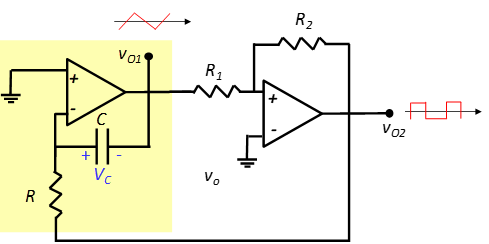
\includegraphics[width=\linewidth]{images/Circuit2.png}
    \caption{Schema circuito}
    \label{fig:Circuit2}
\end{figure}
Il circuito è alimentato dalla tensione duale: $\pm V_{CC}=\pm3V$.\\\\
Il funzionamento per i primi 2 stadi è uguale a quanto detto nel Paragrafo \ref{ch:Spiegazione1}, mentre lo stadio di uscita permette di avere un rendimento migliore di quello ottenuto nell'esperienza precedente. L'efficienza di questo tipo di stadio è dovuta all'attivazione di un solo transistor per semionda. Tuttavia, come si vedrà successivamente, questo circuito ha l'inconveniente di una sensibile distorsione di crossover, dovuta alla soglia di conduzione dei transistor.
\subsection{Assemblaggi e settaggi}
Il circuito in Figura \ref{fig:Circuit2} è stato realizzato modificando direttamente lo schema in classe A (Figura \ref{fig:Circuit1}) con uno stadio in classe B e sostituendo l'integrato MCP6002 con l'integrato TL082CP.\\\\
Lo stadio in classe B push-pull è stato realizzato utilizzando l'accoppiamento di un transistor di potenza NPN $(Q_1)$, codice TIP41CG e un transistor PNP di potenza $(Q_2)$, codice TIP42CG. Le altre componenti sono rimaste invariate dal Primo esperimento\\\\
Il generatore di forma d'onda è stato impostato con il seguente segnale:
\begin{itemize}
    \item Forma d'onda: sinusoidale
    \item Ampiezza iniziale: $100mV$ picco-picco
    \item Frequenza: $330Hz$ (nota Mi)
\end{itemize}
\clearpage
\subsection{Procedura di valutazione e risultati}
Dopo aver acceso l'alimentazione, l'oscilloscopio è stato impostato in modo da visualizzare il segnale di ingresso e il segnale di uscita. Il potenziometro che regola il volume è stato regolato in modo di raggiungere un'ampiezza di $1V_{pp}$ sul segnale di uscita.\\
Si è proseguito a misurare i due segnali con l'oscilloscopio, le cui forme d'onda sono riportare in Figura \ref{fig:scope_9} 
\begin{figure}[H]
    \centering
    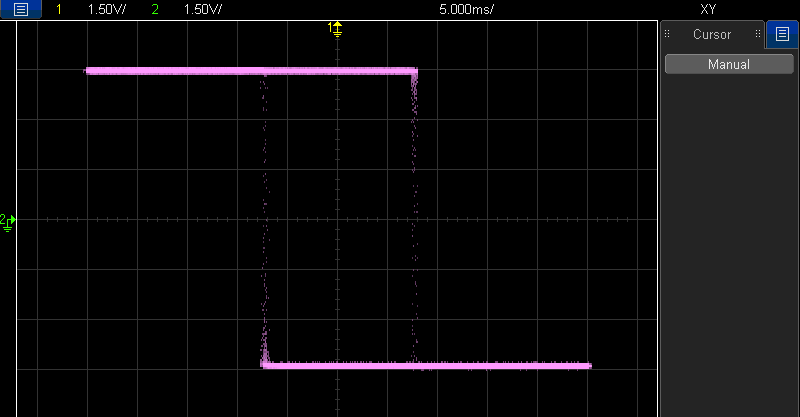
\includegraphics[width=0.7\linewidth]{images/scope_9.png}
    \caption{Segnali di ingresso e uscita dell'amplificatore in classe B}
    \label{fig:scope_9}
\end{figure}
Si è proseguito misurando, attraverso i cursori dell'oscilloscopio, il tempo morto dovuto alla distorsione di crossover.
\begin{equation*}
    \text{Dead time} = 503.125\mu s
\end{equation*}
risultato piùttosto rilevante, considerato che la forma d'onda data in ingresso ha periodo di $T=3\text{ms}$. Si riporta in Figura \ref{fig:scope_11} il dettaglio della distorsione di crossover
\begin{figure}[H]
    \centering
    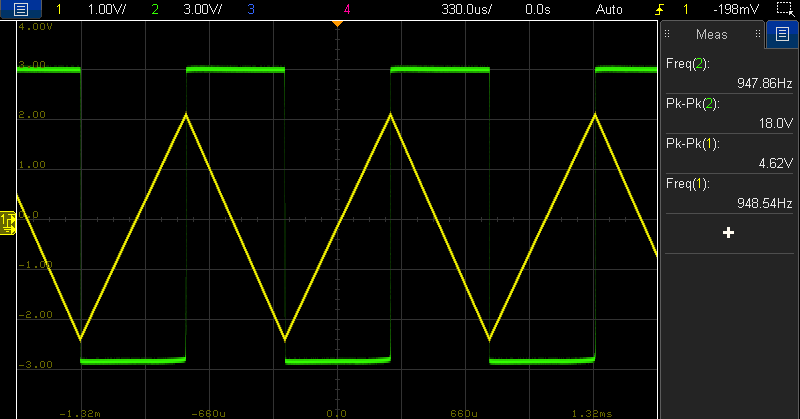
\includegraphics[width=0.7\linewidth]{images/scope_11.png}
    \caption{Dettaglio misurazione distorsione crossover}
    \label{fig:scope_11}
\end{figure}
\subsubsection{Lettore MP3}
Come spiegato nella prima esperienza, si deciso di utilizzare una resistenza di 8$\Omega$ al posto dell'altoparlante, quindi non si è potuto svolgere la prova della riproduzione di una traccia audio. L'obiettivo era quello di sentire l'effetto della distorsione di crossover.
\subsubsection{Commenti}
Le prestazioni di questo amplificatore sono buone, anche se con qualche compromesso. Infatti a livello teorico il rendimento è molto alto, ci sono poce dispersioni di potenza. Come contro, questo circuito ha una distorsione del segnale di uscita decisamente elevata.
    \clearpage
    
    \section{Multivibratore astabile basato su BJT}
    In questo esperimento facoltativo si vuole realizzare un multi vibratore astabile basato su BJT che fa accendere alternativamente due diodi LED, ponendo particolare attenzione a comprenderne e descriverne il funzionamento. Il circuito è riportato in Figura \ref{fig:Circuit_fac}.Sono stati utilizzati i seguenti componenti:
\begin{itemize}
    \item 2 transistor bipolari NPN, codice BC548
    \item Resistenze: $R_1=R_4=470\Omega,R_2=R_3=47\text{k}\Omega$ 
    \item Condensatori: $C_1=C_2=10\mu F$
    \item LED rossi, codice CREE C503B-RCS-CW0Z0AA1
\end{itemize}
Il circuito è alimentato da una tensione $V_{CC}=+12V$ e in Figura \ref{fig:Package3} si è riportato il package del transistor e del led
\begin{figure}[H]
    \centering
    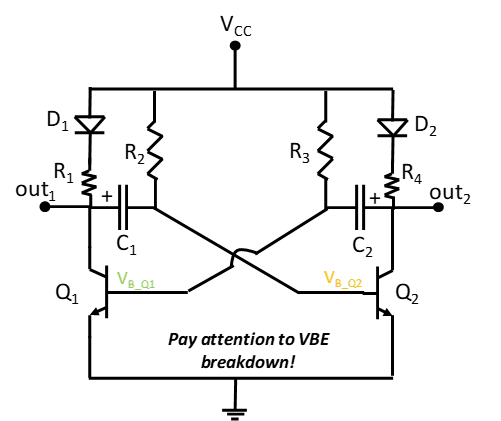
\includegraphics[width=0.5\linewidth]{images/Circuit_fac1.png}
    \caption{Schema circuito}
    \label{fig:Circuit_fac}
\end{figure}
\begin{figure}[H]
    \centering
    \begin{subfigure}{.5\textwidth}
      \centering
      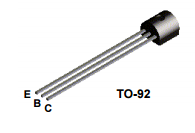
\includegraphics[width=0.5\linewidth]{images/BC548.png}
    \end{subfigure}%
    \begin{subfigure}{.5\textwidth}
      \centering
      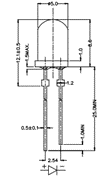
\includegraphics[width=0.3\linewidth]{images/LED.png}
    \end{subfigure}
    \caption{Package del BJT BC548 e del LED}
    \label{fig:Package3}
\end{figure}

\subsection{Risultati}
\subsubsection*{Misurare le forme d’onda alla base e al collettore del transistor $Q_1$ e riportarle in relazione}
Con l'utilizzo dell'oscilloscopio è stato campionato il segnale e  ottenuto le seguenti forme d'onda, riportate in Figura \ref{fig:FacBaseQ1} per la misura alla base e in Figura \ref{fig:FacCollectorQ1} per la misura al collettore.
\begin{figure}[H]
    \centering
    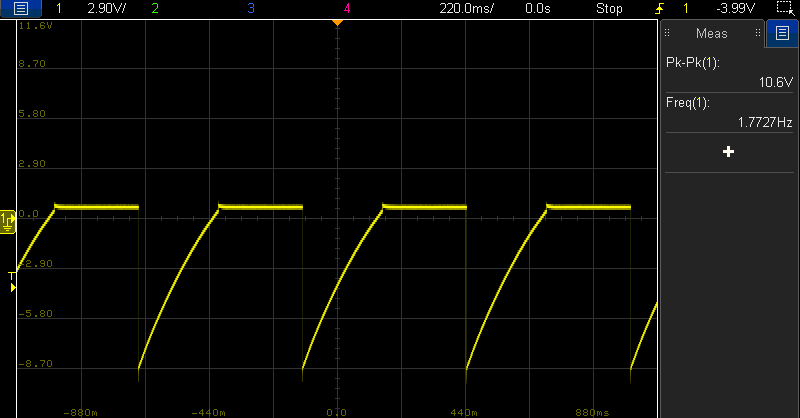
\includegraphics[width=0.7\linewidth]{images/scope_20.png}
    \caption{Forma d'onda campionata alla base di $Q_1$}
    \label{fig:FacBaseQ1}
\end{figure}
\begin{figure}[H]
    \centering
    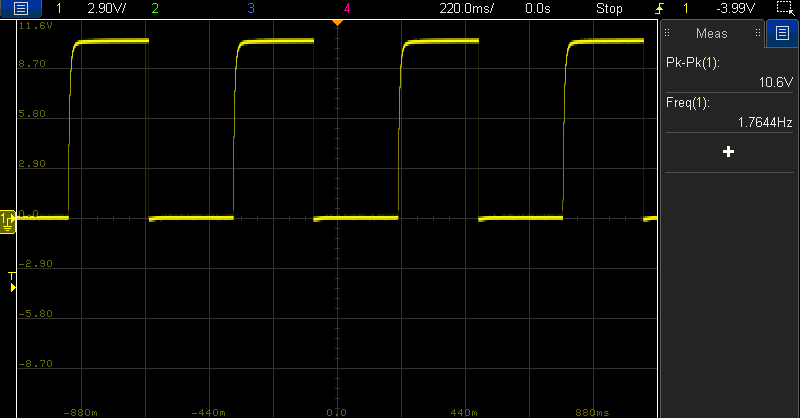
\includegraphics[width=0.7\linewidth]{images/scope_22.png}
    \caption{Forma d'onda campionata al collettore di $Q_1$}
    \label{fig:FacCollectorQ1}
\end{figure}
\subsubsection*{Riportare il confronto della forma d’onda $out_1$ e $out_2$ in relazione}
Sempre con l'utilizzo dell'oscilloscopio è stato campionato il canale di entrambe le uscite per poi metterle a confronto in Figura \ref{fig:FacConfronto}
\begin{figure}[H]
    \centering
    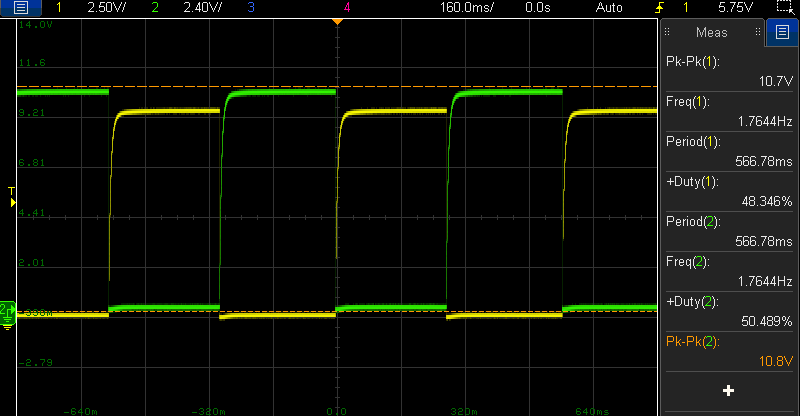
\includegraphics[width=0.7\linewidth]{images/scope_26.png}
    \caption{Confronto della forma d’onda $out_1$ e $out_2$}
    \label{fig:FacConfronto}
\end{figure}
\subsubsection*{Valutare il periodo, frequenza e duty cycle della forma d’onda generata all’uscita $out_1$ e $out_2$}
L'oscilloscopio fornisce i seguenti parametri delle forme d'onda generate dal circuito, riassunti nella Tabella \ref{tab:RisFac1}
\begin{table}[H]
    \centering
    \begin{tabular}{||c|c|c|c|c||}
        \hline\hline
        Uscita & Vpp & Periodo & Frequenza & Duty cycle \\\hline
        $out_1$ & 10.7V & 566.78ms & 1.7644Hz & 48.346\% \\\hline
        $out_2$ & 10.8V & 566.78ms & 1.7644Hz & 50.489\%\\\hline
    \end{tabular}
    \caption{Valutazione dei segnali di uscita}
    \label{tab:RisFac1}
\end{table}
\subsection{Funzionamento del circuito} 

Un circuito multivibratore astabile basato su transistor BJT è costituito da due BJT, due condensatori, due diodi e quattro resistenze, tali che $R_1=R_2<R_2=R_3$. Il circuito funziona in modo che i due transistor si alternino nel loro stato di accensione e spegnimento. Entrambi i transistor sono accoppiati a croce, ciò significa che il collettore di un transistor è connesso alla base dell'altro transistor attraverso una capacità.
Nel momento in cui viene fornita l'alimentazione, uno dei due transistor si accende più rapidamente dell'altro a causa di piccole differenze tra i dispositivi. Supponendo che $Q_1$ vada in saturazione per primo, la tensione base-emettitore di $Q_1$ si porta al valore di $0.7V$ e la tensione al collettore di $Q_2$ si porta al potenziale di massa. Questo comporta che alla base di $Q_2$ appare l'inverso della tensione ai capi del condensatore $C_1$, portandolo nella regione di interdizione (cut-off), di conseguenza al collettore di $Q_2$ si ha il potenziale $V_{cc}$. 
Si ha $Q_1$ On e $Q_2$ Off.\\\\
Il condensatore $C_2$ inizia a caricarsi fino al potenziale $V_{cc}-V_{be}$, mentre il condensatore $C_1$ fino a $V_{cc}$. Dato $R_1<R_2$ si ha che $C_2$ si carica più rapidamente di $C_1$.
Appena la tensione ai capi di $C_1$ (e quindi alla base di $C_2$) diventa $0.7V$ il transistor $Q_2$ inizia a condurre fino a entrare in saturazione. Di conseguenza la tensione al collettore di $Q_2$ si porta al potenziale di massa. La tensione alla base di $Q_1$ si porta all'inverso del valore ai capi di $C_2$, quindi a $-(V_{cc} - V_{be})$ e $Q_1$ entra in interdizione.
Si ha $Q_1$ Off e $Q_2$ On.\\\\
Da qui in poi il circuito continuerà a cambiare tra i due stati fino alla rimozione dell'alimentazione.
\subsection{Periodo della forma d’onda}
Il periodo $T$ della forma d'onda dipende dalle resistenze $R_2$ e $R_3$ e dai condensatori $C_1$ e $C_2$ utilizzati nel circuito, secondo la formula:
\begin{equation}
    T=\ln{2}(R_2C_1+R_3C_2)
\end{equation}

    \clearpage

    \section{Oscillatore a rilassamento}
    In questa esperimento facoltativo è stato descritto e in seguito analizzato il funzionamento dell'oscillatore a rilassamento. Il circuito è rappresentato in Figura \ref{fig:Circuit_FAC2}. Sono stati utilizzati i seguenti componenti:
\begin{itemize}
    \item Amplificatore operazionale a doppia uscita, codice TL082CP
    \item Resistenze $R_1,R_2,R$ a valori da determinare
    \item Condensatore da $100nF,220nF,1\mu F$ in dotazione
\end{itemize}
\begin{figure}[H]
    \centering
    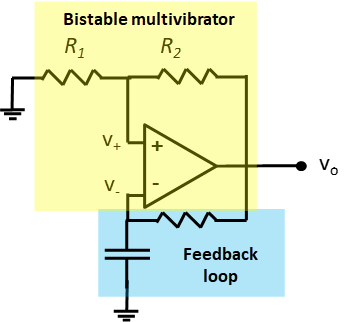
\includegraphics[width=0.6\linewidth]{images/Circuit_fac2.png}
    \caption{Schema circuito}
    \label{fig:Circuit_FAC2}
\end{figure}
Il circuito è alimentato dalla tensione duale: $\pm V_{CC}=\pm10V$
\subsection{Descrizione del funzionamento del circuito}
Un modo semplice per generare onde quadre è forzare un circuito bistabile a cambiare stato periodicamente. Questo può essere ottenuto connettendo un circuito bistabile a una rete di retroazione RC. Questo circuito non ha stati stabili, ed è detto multivibratore astabile.

Si noti che non sono presenti ingressi, ciò comporta che all'accensione dell'alimentazione l'uscita $V_o$ si porta a uno dei due valori di saturazione $L_+$ o $L_-$.
Se per ipotesi l'uscita si trova al valore $L_+$, si ha $V_+=\beta L_+$ (con $\beta = \frac{R1}{R1+R2}$), mentre il condensatore $C$ si carica verso L+ attraverso la resistenza $R$. 
Quando la tensione ai capi del condensatore raggiunge $V_{th}=\beta L_+$, l'uscita $V_o$ commuta verso l'altro stato stabile in cui $V_o = L_-$ e $V_+ =\beta L_-$.
Il condensatore inizia a scaricarsi fino a $V_{tl} = \beta L_-$, dove avviene la successiva commutazione.
Da qui in poi il circuito continua a commutare tra i due stati fino allo spegnimento dell'alimentazione.
\subsection{Dimensionamento del circuito}
Si vuole dimensionare i  componenti $R_1,R_2,R,C$, in modo tale che il circuito risultante abbia frequenza di oscillazione pari a $100Hz$.\\
Il periodo $T$ dell'onda quadra in uscita vale
\begin{equation}
    T=2\tau\ln{\frac{1+\beta}{1-\beta}}
\end{equation}
Dove $\beta=R_1/R_1+R_2$ e $\tau=RC$ costante di tempo. I valori di $R_1,R_2$ sono quelli scelti nel primo esperimento, quindi
\begin{equation*}
    R_1=R_2=10k\Omega\implies\frac{1+\beta}{1-\beta}=3
\end{equation*}
Scelto un valore di capacità tra quelli disponibili, è stato ricavato il valore della resistenza $R$ da
\begin{equation}
    R=\frac{1}{f2C\ln{3}}
\end{equation}
Quindi ponendo $C=100nF$ si è ottenuto
\begin{equation*}
    R = 45511.96\Omega \approx 47k\Omega
\end{equation*}
Riassumiamo nella tabella sotto il dimensionamento del circuito scelto.
\begin{table}[H]
    \centering
    \begin{tabular}{|c|c|}
        \hline
        $R_1$&$10k\Omega$\\\hline
        $R_2$&$10k\Omega$\\\hline
        $R$&$47k\Omega$\\\hline
        $C$&$100nF$\\\hline
    \end{tabular}
\end{table}
\subsection{Risultati}
Sono riportate di seguito le forme d'onda di $v_0,v_{-},v_{+}$, rispettivamente in Figura \ref{fig:FACV0},\ref{fig:FACV-},\ref{fig:FACV+}.
\begin{figure}[H]
    \centering
    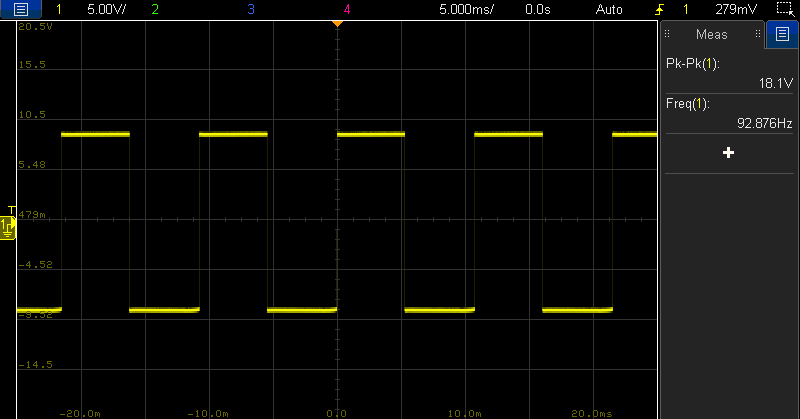
\includegraphics[width=0.7\linewidth]{images/FACV0.png}
    \caption{Forma d'onda presa in $v_0$}
    \label{fig:FACV0}
\end{figure}
\begin{figure}[H]
    \centering
    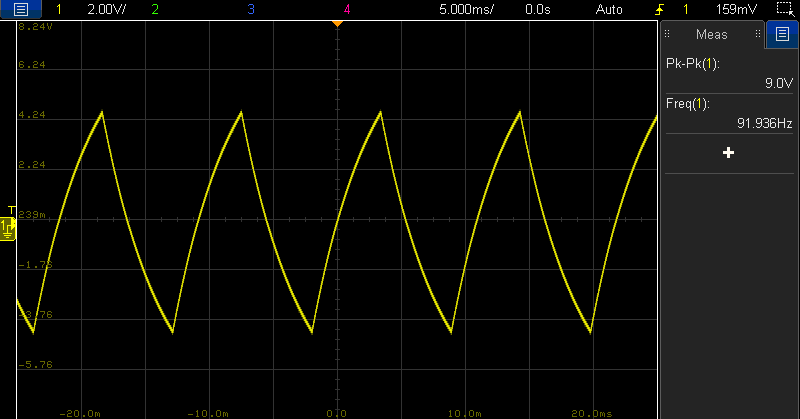
\includegraphics[width=0.7\linewidth]{images/FACV-.png}
    \caption{Forma d'onda presa in $v_-$}
    \label{fig:FACV-}
\end{figure}
\begin{figure}[H]
    \centering
    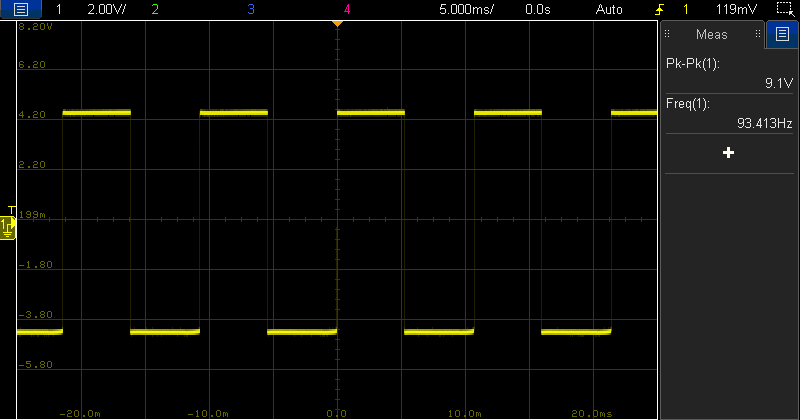
\includegraphics[width=0.7\linewidth]{images/FACV+.png}
    \caption{Forma d'onda presa in $v_+$}
    \label{fig:FACV+}
\end{figure}
\clearpage
\subsection{Elaborazione dati con MATLAB\textregistered\xspace}
Riportiamo in Figura \ref{fig:MatlabPlot} il plotting fatto con MATLAB\textregistered\xspace dei dati campionati con l'oscilloscopio.
\begin{figure}[H]
    \centering
    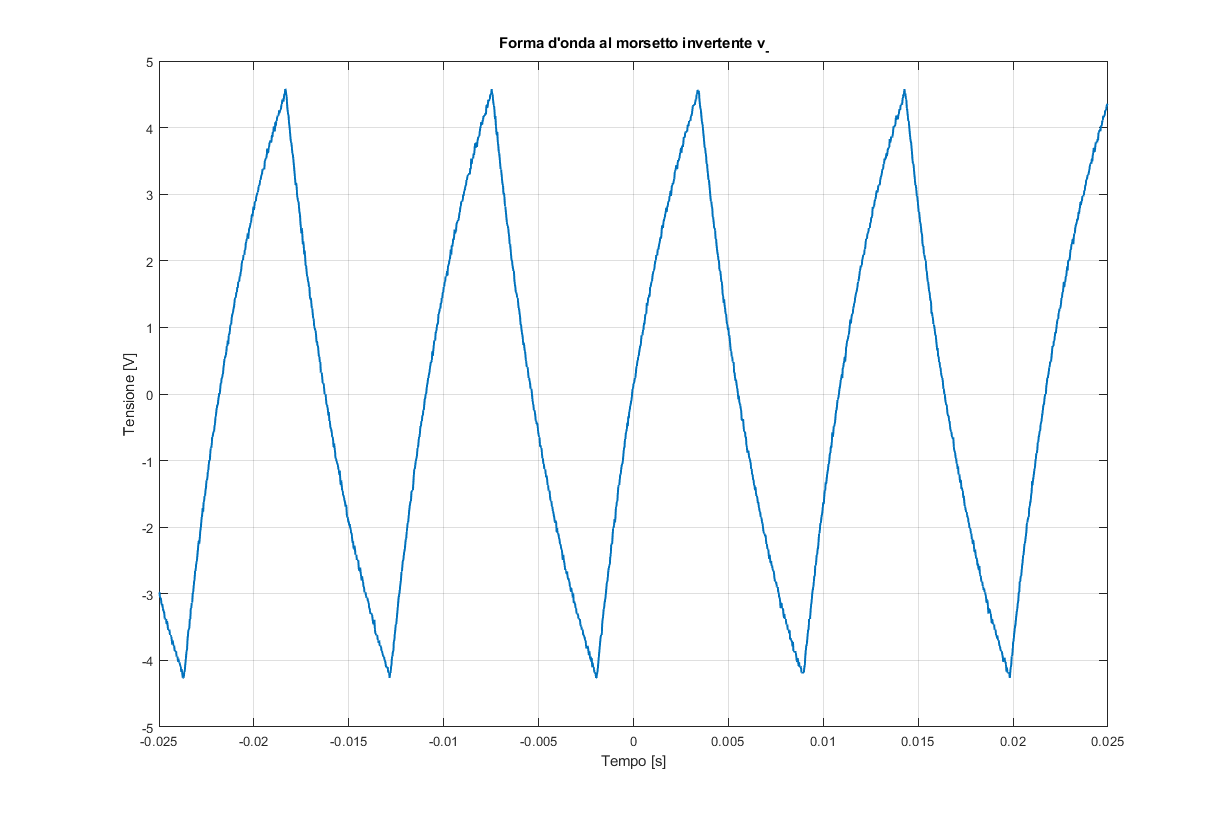
\includegraphics[width=0.6\linewidth]{images/MatlbFac2.png}
    \caption{Plot MATLAB\textregistered\xspace}
    \label{fig:MatlabPlot}
\end{figure}
Il valore di $\tau$ determinato dal dimensionamento del circuito è
\begin{equation*}
    \tau=RC=0.0047 \quad[\Omega F]
\end{equation*}
Tramite la funzione \textit{CurveFitter} di MATLAB\textregistered\xspace abbiamo ricavato un valore alla variabile $\tau$. Il fitting è stato fatto solo su un fronte di salita scelto. Come si vede in Figura \ref{fig:MatlabFit}
\begin{figure}[H]
    \centering
    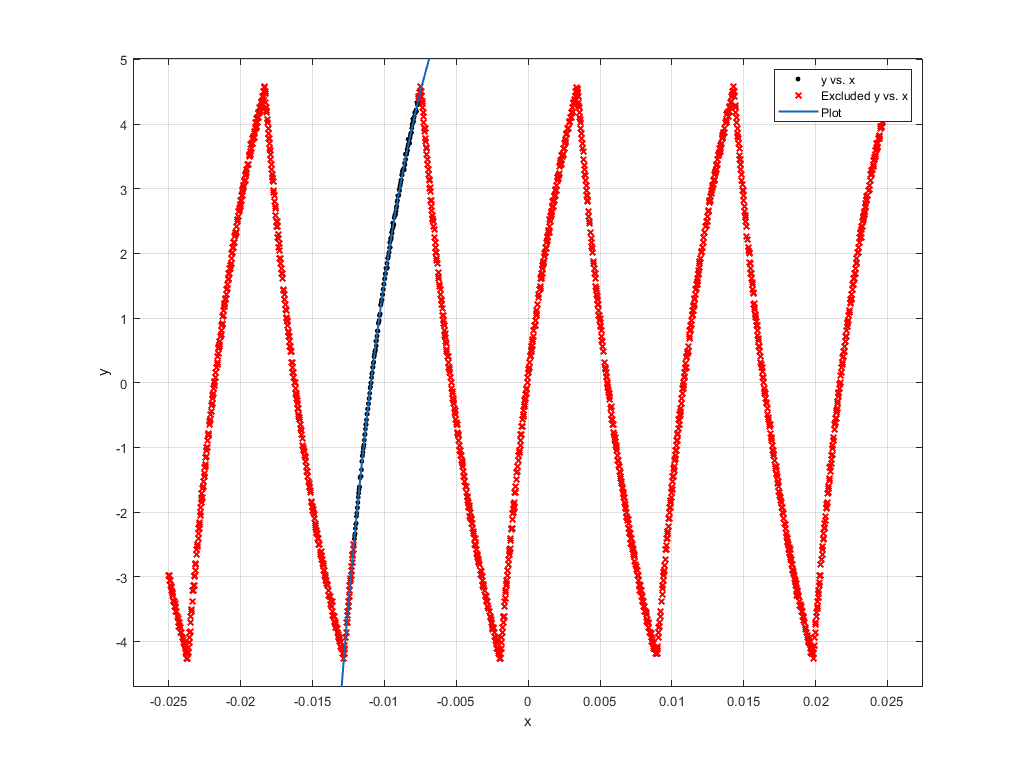
\includegraphics[width=0.6\linewidth]{images/MatlbFIT curve.png}
    \caption{Curve Fitter sui dati campionati}
    \label{fig:MatlabFit}
\end{figure}
Dal fitting abbiamo ricavato il seguente valore di $\tau = 0.004707$.
\end{document}
